\section{Результаты измерений}
\addcontentsline{toc}{section}{Результаты измерений}	% Добавляем его в оглавление

\begin{enumerate}
\item 
Измерить силу постоянных токов протекающих через нагрузки, с помощью приборов Ц4353 и М92А. Оценить инструментальную и методическую погрешности измерения тока.

\begin{figure}[h]
  \begin{minipage}[h]{0.4\linewidth}
    \center{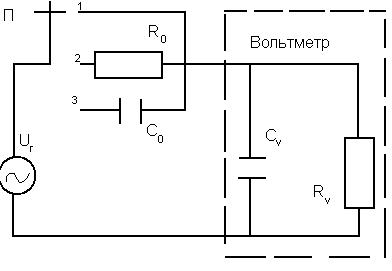
\includegraphics[width=1\linewidth]{scheme1} \\ а)}
  \end{minipage}
  \hfill
  \begin{minipage}[h]{0.4\linewidth}
    \center{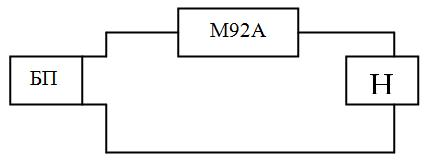
\includegraphics[width=1\linewidth]{scheme2} \\ б)}
  \end{minipage}
  \caption{Схемы установок}
\end{figure}

\hspace{4mm}



\begin{table} [htbp]
  \centering
  \begin{tabular}{| p{1cm} | p{2cm} | p{2cm} | p{2cm} | p{1.5cm} | p{1.5cm} | p{1.5cm} | p{1.5cm}l |}
  \hline
  \centering Ц4353 &\centering Номер нагрузки &\centering Предел измерения &\centering $ I_{i}, $ (мА) &\centering $ \delta_{i}$ , \%  &\centering $ \delta_{mi} $, \% &\centering $ q_{i} $, мА &\centering $ I $, мА &\\ \cline{2-9}
  &\centering &\centering &\centering &\centering &\centering &\centering &\centering  &\\ \cline{2-9}
  &\centering &\centering &\centering &\centering &\centering &\centering &\centering  &\\ \cline{2-9}
  \hline

  \centering M92A &\centering Номер нагрузки &\centering Предел измерения &\centering $ I_{i}, $ (мА) &\centering $ \Delta_{i}$ , \%  &\centering $ \delta_{mi} $, \% &\centering $ q_{i} $, мА &\centering $ I $, мА &\\ \cline{2-9}
  &\centering &\centering &\centering &\centering &\centering &\centering &\centering  &\\ \cline{2-9}
  &\centering &\centering &\centering &\centering &\centering &\centering &\centering  &\\ \cline{2-9}
  \hline
  \end{tabular}
  \caption{Результаты измерений силы постоянных токов}
\end{table}

\clearpage

\item
Измерить сопротивления, воспроизводимые магазином МСП-63, с помощью приборов Ц4353 и М92А. Оценить методическую погрешность измерения сопротивления.


\begin{figure}[h]
  \begin{minipage}[h]{0.4\linewidth}
    \center{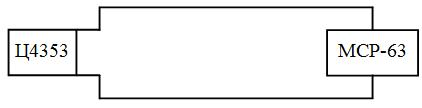
\includegraphics[width=1\linewidth]{scheme3} \\ а)}
  \end{minipage}
  \hfill
  \begin{minipage}[h]{0.4\linewidth}
    \center{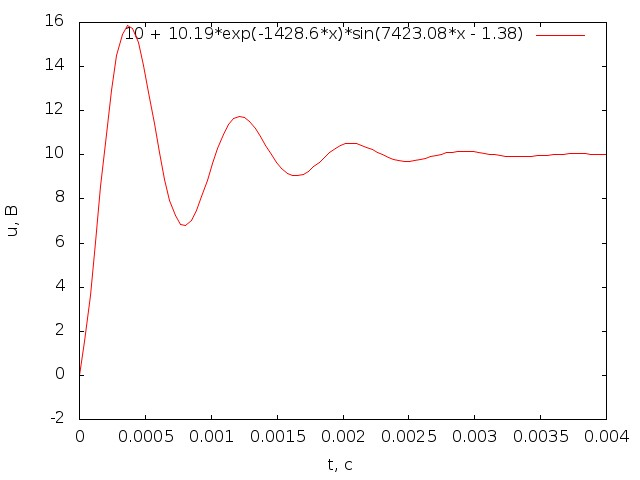
\includegraphics[width=1\linewidth]{scheme4} \\ б)}
  \end{minipage}
  \caption{Схемы установок}
\end{figure}

\vspace{4mm}

\begin{table} [htbp]
  \centering
  \begin{tabular}{| p{1cm} | p{2cm} | p{2cm} | p{2cm} | p{1.5cm} | p{1.5cm} | p{1.5cm} | p{2cm}l |}
  \hline
  \centering Ц4353 &\centering $ R_{mc} $, кОм &\centering Предел измерения &\centering $ R_{i} $, кОм &\centering $ \delta_{rmc} $ , \%  &\centering $ \Delta_{rmc} $, \% &\centering $ \delta_{r} $, \% &\centering $ \Delta_{r} $, кОм &\\ \cline{2-9}
  &\centering &\centering &\centering &\centering &\centering &\centering &\centering &\\ \cline{2-9}
  &\centering &\centering &\centering &\centering &\centering &\centering &\centering &\\ \cline{2-9}
  &\centering &\centering &\centering &\centering &\centering &\centering &\centering &\\ \cline{2-9}
  \hline
  \centering M92A &\centering $ R_{mc} $, кОм &\centering Предел измерения & \multicolumn{2}{c|}{ $ R_{u} $, кОм } & \multicolumn{4}{c|}{ $\delta_{r}$ , кОм } \\ \cline{2-9}
  &\centering &\centering &\multicolumn{2}{c|}{} & \multicolumn{4}{c|}{ } \\ \cline{2-9}
  &\centering &\centering &\multicolumn{2}{c|}{} & \multicolumn{4}{c|}{ } \\ \cline{2-9}
  &\centering &\centering &\multicolumn{2}{c|}{} & \multicolumn{4}{c|}{ } \\ \cline{2-9}
  \hline
  \end{tabular}
  \caption{Результаты измерений сопротивления}
\end{table}

\clearpage

\item
Провести поверку прибора Ц4353 в части определения погрешности измерения напряжения постоянного тока при использовании прибора В7-34. Оценить абсолютную, относительную и приведенную погрешности прибора Ц4353 при измерении напряжения постоянного тока. 
x
\begin{figure} [h] 
  \center
  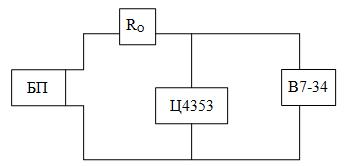
\includegraphics [width=0.5\linewidth] {scheme5}
  \caption{Схема установки} 
\end{figure}

\vspace{4mm}

\begin{table} [htbp]
  \centering
  \begin{tabular}{| p{1.5cm} | p{1.5cm} | p{1.5cm} | p{1.5cm} | p{1.5cm} | p{1.5cm} | p{1.5cm} | p{1.5cm}l |}
  \hline
  \centering № п/п &\centering $ U $, В &\centering $ U_{0} $. В &\centering $ \Delta_{u} $, В &\centering $ \delta_{u} $, \% &\centering $ \gamma_{u}$ , \%  &\centering $ \delta_{oi} $, \% &\centering $ \Delta_{oi} $, В &\\
  \hline
  \centering 1 &\centering &\centering &\centering &\centering &\centering &\centering &\centering &\\
  \hline
  \centering 2 &\centering &\centering &\centering &\centering &\centering &\centering &\centering &\\
  \hline
  \centering 3 &\centering &\centering &\centering &\centering &\centering &\centering &\centering &\\
  \hline
  \end{tabular}
  \caption{Результаты поверки прибора Ц4353}	
\end{table}

Предел измерений -- 15 В.

\end{enumerate}
\clearpage
